\documentclass[8pt,a4paper,compress]{beamer}

\usepackage{/home/siyer/lib/slides}

\title{Case Study: Union-Find}
\date{}

\begin{document}
\begin{frame}
\vfill
\titlepage
\end{frame}

\begin{frame}
\frametitle{Outline}
\tableofcontents
\end{frame}

\section{The Dynamic Connectivity Problem}
\begin{frame}[fragile]
\begin{minipage}{250pt}
\begin{itemize}
\item consider an input sequence of pairs of integers, where each integer represents an object of some type, and the pair $(p, q)$ means that ``$p$ is connected to $q$''

\item we assume that ``is connected to'' is an equivalence relation

\item two objects belong to an equivalence class if and only if they are connected

\item the goal of the dynamic connectivity problem is to devise a data structure to decide whether or not a new pair of objects is connected 

\item applications
\begin{itemize}
\item determine if two vertices in a network are connected

\item determine if two variable names in a computer program are equivalent, ie, refers to the same object

\item if we think of the integers as belonging to mathematical sets, when we process a pair $(p, q)$, we are asking whether they belong to the same set, and if not, we unite $p$'s set and $q$'s set, putting them in the same set
\end{itemize}
\end{itemize}
\end{minipage}%
\begin{minipage}{60pt}
\hfill 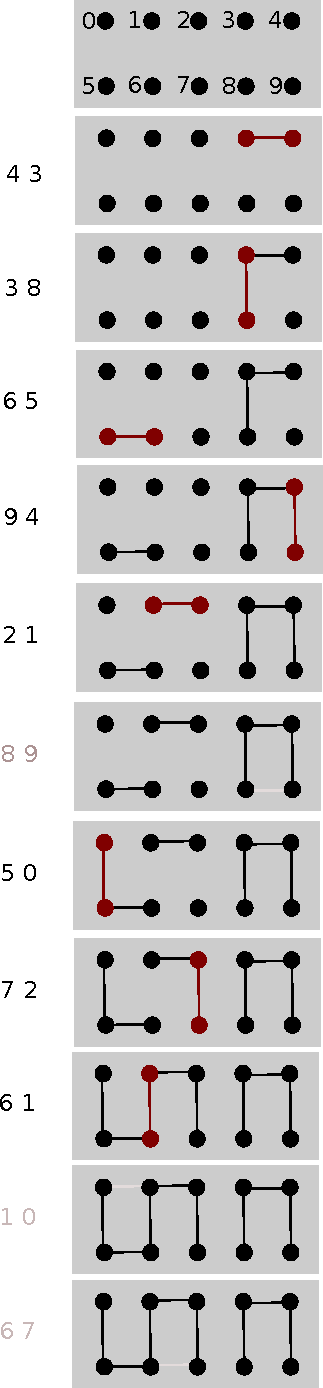
\includegraphics[scale=0.35]{./figures/dyn_conn.pdf}
\end{minipage}
\end{frame}

\begin{frame}[fragile]
\begin{itemize}
\item following network terminology, we refer to the objects as sites, the pairs as connections, and the equivalence classes as connected components, or just components for short

\item for simplicity, we assume that we have $N$ sites with integer names, from 0 to $N-1$

\item the union-find API
\begin{lstlisting}[language={},mathescape]
public interface UF

    int find(int p)          // component identifier for $p$ (0 to $N-1$)
    int count()              // number of components
    boolean connected(int p, int q) // are $p$ and $q$ in the same component?
    void union(int p, int q)        // add connection between $p$ and $q$
\end{lstlisting} 
\end{itemize}
\end{frame}

\begin{frame}[fragile]
\begin{minipage}{250pt}
\begin{itemize}
\item \lstinline{UF} client
\begin{lstlisting}[language=Java]
public class QuickFindUF implements UF {
    ...
    public static void main(String[] args) {
        int N = StdIn.readInt();
        QuickFindUF uf = new QuickFindUF(N);
        while (!StdIn.isEmpty()) {
            int p = StdIn.readInt();
            int q = StdIn.readInt();
            if (uf.connected(p, q)) { continue; }
            uf.union(p, q);
            StdOut.println(p + " " + q);
        }
        StdOut.println(uf.count() + " components");
    }
}
\end{lstlisting}
    
\begin{lstlisting}[language={}]
$ more tinyUF.txt
10
4 3 3 8 6 5 9 4 2 1 8 9 5 0 7 2 6 1 1 0 6 7
\end{lstlisting}    

\begin{lstlisting}[language={}]
$ java QuickFindUF < tinyUF.txt 
4 3
3 8
6 5
9 4
2 1
5 0
7 2
6 1
2 components
\end{lstlisting}
\end{itemize}
\end{minipage}%
\begin{minipage}{60pt}
\hfill 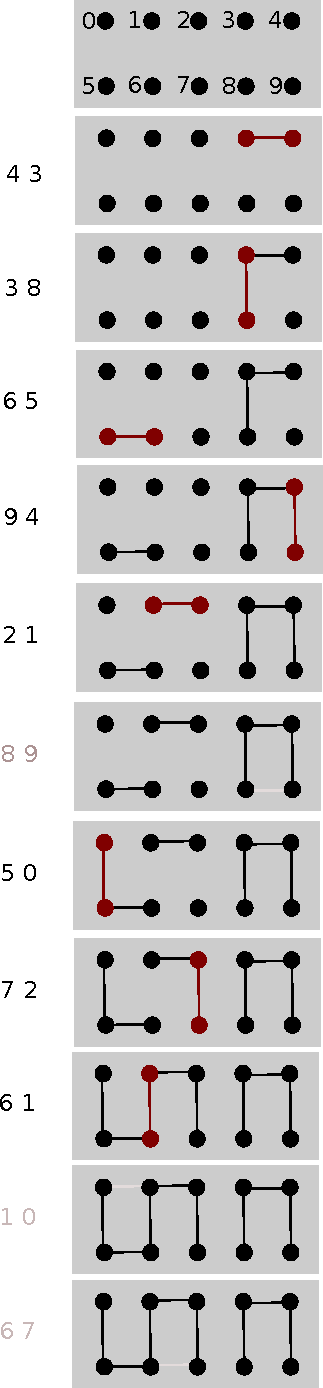
\includegraphics[scale=0.35]{./figures/dyn_conn.pdf}
\end{minipage}
\end{frame}

\section{Quick-find}
\begin{frame}[fragile]
\begin{itemize}
\item \lstinline{UF} implementation
\begin{lstlisting}[language=Java]
public class QuickFindUF implements UF {
    private int[] id; 
    private int count; 

    public QuickFindUF(int N) {
        count = N;
        id = new int[N];
        for (int i = 0; i < N; i++) { 
            id[i] = i; 
        }
    }

    public int find(int p) { return id[p]; }

    public int count() { return count; }
  
    public boolean connected(int p, int q) { return find(p) == find(q); }

    public void union(int p, int q) {
        int i = find(p);
        int j = find(q);
        if (i == j) { return; }
        for (int k = 0; k < id.length; k++) {
            if (id[k] == i) { 
                id[k] = j; 
            }
        }
        count--; 
    }
    ...
}
\end{lstlisting}
\end{itemize}
\end{frame}

\section{Quick-union}
\begin{frame}[fragile]
\begin{itemize}
\item \lstinline{UF} implementation
\begin{lstlisting}[language=Java]
public class QuickUnionUF {
    private int[] id;
    private int count;

    public QuickUnionUF(int N) {
        count = N;
        id = new int[N];
        for (int i = 0; i < N; i++) { id[i] = i; }
    }

    public int find(int p) {
        while (p != id[p]) { p = id[p]; }
        return p;
    }

    public int count() { return count; }

    public boolean connected(int p, int q) { return find(p) == find(q); }

    public void union(int p, int q) {
        int i = find(p);
        int j = find(q);
        if (i == j) { return; }
        id[i] = j;
        count--;
    }
    ...
}
\end{lstlisting}
\end{itemize}
\end{frame}

\section{Weighted Quick-union}
\begin{frame}[fragile]
\begin{itemize}
\item \lstinline{UF} implementation
\begin{lstlisting}[language=Java]
public class WeightedQuickUnionUF {
    private int[] id; 
    private int[] sz; 
    private int count; 

    public WeightedQuickUnionUF(int N) {
        count = N;
        id = new int[N];
        sz = new int[N];
        for (int i = 0; i < N; i++) {
            id[i] = i;
            sz[i] = 1;
        }
    }

    public int count() { return count; }

    public int find(int p) {
        while (p != id[p]) { p = id[p]; }
        return p;
    }

    public boolean connected(int p, int q) { return find(p) == find(q); }

    public void union(int p, int q) {
        int i = find(p);
        int j = find(q);
        if (i == j) { return; }
        if (sz[i] < sz[j]) { id[i] = j; sz[j] += sz[i]; }
        else { id[j] = i; sz[i] += sz[j]; }
        count--;
    }
    ...
}
\end{lstlisting}
\end{itemize}
\end{frame}

\section{Performance Characteristics of Union-find Algorithms}
\begin{frame}[fragile]
\begin{itemize}
\item dynamic connectivity experiments
\begin{center}
\begin{tabular}{p{3cm}ccc}
\centering \textbf{algorithm} & \textbf{$N=10$} & \textbf{$N=625$} & \textbf{$N=10^6$} \\ \hline \\
\centering quick-find & 0.112s & 0.175s & 14m49.525s \\
\centering quick-union & 0.113s & 0.175s & 134m5.980s \\
\centering weighted quick-union & 0.125s & 0.204s & 6.718s
\end{tabular} 
\end{center}

\item worst-case order of growth for $N$ sites
\begin{center}
\begin{tabular}{p{3cm}ccc}
\centering \textbf{algorithm} & \textbf{constructor} & \textbf{union} & \textbf{find} \\ \hline \\
\centering quick-find & $N$ & $N$ & 1 \\
\centering quick-union & $N$ & tree height & tree height \\
\centering weighted quick-union & $N$ & $\log N$ & $\log N$ \\
\centering weighted quick-union with path compression & $N$ & $\approx 1$ (amortized) & $\approx 1$ (amortized) \\
\centering impossible & $N$ & 1 & 1
\end{tabular} 
\end{center}
\end{itemize}
\end{frame}

\end{document}
